\documentclass[table]{beamer}  


%\usepackage{beamerthemesplit}

%\usepackage{colortbl}
%\usepackage{algorithm, algorithmic}
%\usepackage{tikz}
\usepackage[BoldFont,SlantFont,CJKchecksingle]{xeCJK}
\usepackage{graphicx}
\usepackage{multicol}
\usepackage{amsmath}

\setCJKmainfont[BoldFont=SimHei,SlantedFont=KaiTi]{SimSun}
\setCJKsansfont[BoldFont=SimHei,SlantedFont=KaiTi]{SimSun}
\setCJKmonofont[ItalicFont={Adobe Fangsong Std}]{SimSun}
\setCJKfamilyfont{zhsong}{SimSun}
\setCJKfamilyfont{zhhei}{SimHei}
\setCJKfamilyfont{zhkai}{KaiTi}
\setCJKfamilyfont{zhfs}{FangSong}
\usetheme{CambridgeUS}  
\parindent 2em 

  
%\usepackage{fontspec}  

\title{人工神经网络}   
\author{肖强 \ 张哲槟\\密尚华}
\institute{}

\begin{document}  
  
\begin{frame}
\titlepage
\end{frame}

\begin{frame}
	\frametitle{内容}
	
	\begin{multicols}{2}
		\tableofcontents
	\end{multicols}
%\tableofcontents
\end{frame}

\section{人工神经网络简介}

\begin{frame} 
\frametitle{人工神经网络(Artificial Neural Network,ANN )}  
\begin{columns}

\column{.5\textwidth}
神经网络是一种运算模型,由大量的节点(或称神经元)之间相互联接构成。
%每个节点代表一种特定的输出函数,称为激励函数(activation function)。每两个节点间的连接都代表一个对于通过该连接信号的加权值,称之为权重,这相当于人工神经网络的记忆。网络的输出则依网络的连接方式,权重值和激励函数的不同而不同。
\\ 网络自身通常都是对自然界某种算法或者函数的逼近,也可能是对一种逻辑策略的表达。

\column{.5\textwidth}
	\begin{figure}[ht]
	\centering
	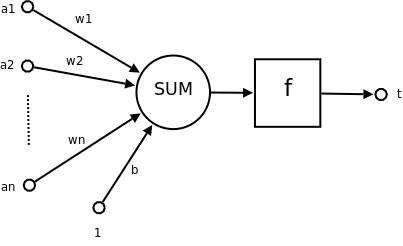
\includegraphics[width=\linewidth]{partition/img/Ncell.png}  
%	\caption{this is a figure demo}
%	\label{fig:label}
	\end{figure}


\end{columns}


\end{frame}  

%topics
\section{SVM}

\begin{frame}
	
  \centerline{\textbf{\Huge{SVM}}}
           
	\begin{figure}[ht]
	\centering
	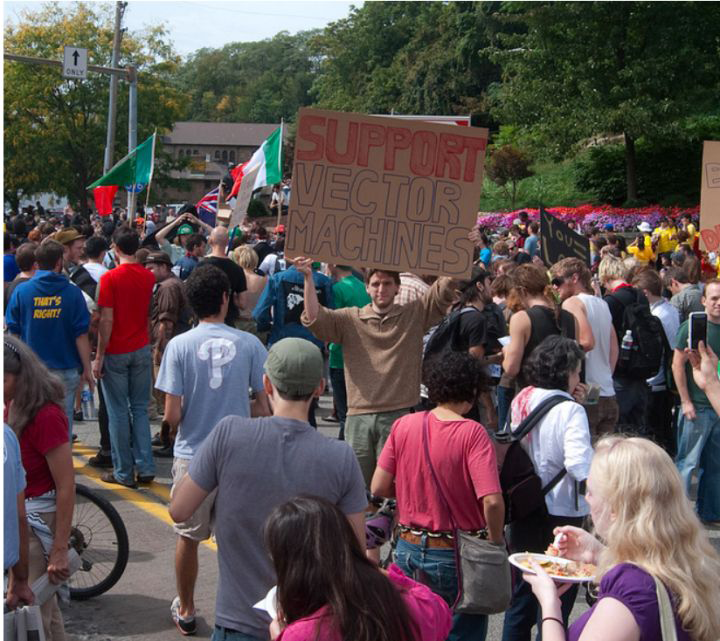
\includegraphics[width=0.5\linewidth]{partition/img/svm_0.png}  
%	\caption{this is a figure demo}
%	\label{fig:label}
	\end{figure}

\end{frame} 

\begin{frame} 
\frametitle{支持向量机}  
\begin{columns}

\column{.5\textwidth}
	\begin{itemize}
		\item SVM, 俗称支持向量机,为一种supervised learning算法,属于classification的范畴。
		\item 在数据挖掘的应用中,与unsupervised的Clustering相对应和区别。
		\item 广泛应用于机器学习(Machine Learning), 计算机视觉(Computer Vision) 和数据挖掘(Data Mining)当中。	
	\end{itemize}

\column{.5\textwidth}
	\begin{figure}[ht]
	\centering
	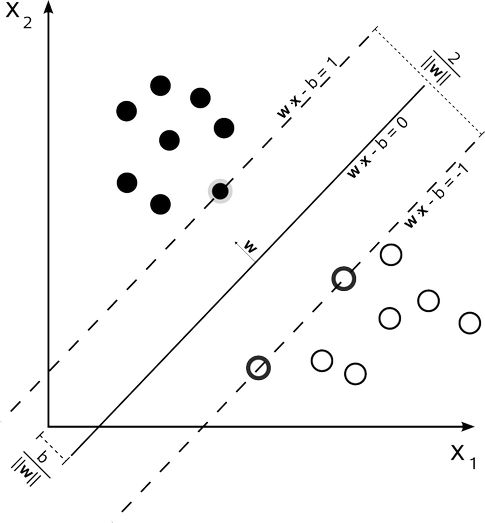
\includegraphics[width=\linewidth]{partition/img/svm_1.jpg}  
%	\caption{this is a figure demo}
%	\label{fig:label}
	\end{figure}


\end{columns}
\end{frame} 

\begin{frame}
\frametitle{一个游戏}	
现在桌子上有两种颜色的球,现在要把他们分开。
           
	\begin{figure}[ht]
	\centering
	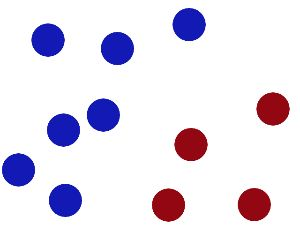
\includegraphics[width=0.5\linewidth]{partition/img/svm_2.jpg}  
%	\caption{this is a figure demo}
%	\label{fig:label}
	\end{figure}

\end{frame} 

\begin{frame}
\frametitle{一个游戏}	
我们把一根棍子放在中间,看上去干得不错。
           
	\begin{figure}[ht]
	\centering
	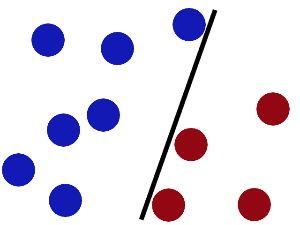
\includegraphics[width=0.5\linewidth]{partition/img/svm_3.jpg}  
%	\caption{this is a figure demo}
%	\label{fig:label}
	\end{figure}

\end{frame} 

\begin{frame}
\frametitle{一个游戏}	
有些人又往桌子上放了一些球,大部分都分对了,但是出现了一个错分的。
           
	\begin{figure}[ht]
	\centering
	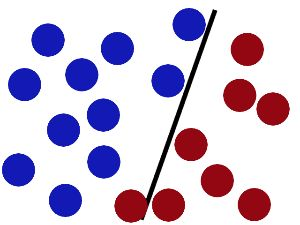
\includegraphics[width=0.5\linewidth]{partition/img/svm_4.jpg}  
%	\caption{this is a figure demo}
%	\label{fig:label}
	\end{figure}

\end{frame} 

\begin{frame}
\frametitle{一个游戏}	
SVM就是试图把棍放在最佳位置,好让在棍的两边有尽可能大的间隙。
           
	\begin{figure}[ht]
	\centering
	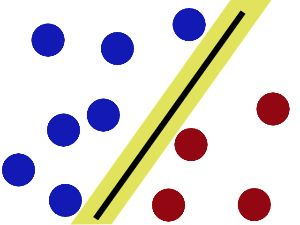
\includegraphics[width=0.5\linewidth]{partition/img/svm_5.jpg}  
%	\caption{this is a figure demo}
%	\label{fig:label}
	\end{figure}

\end{frame} 

\begin{frame}
\frametitle{一个游戏}	
现在即使放了更多的球,棍仍然是一个好的分界线
           
	\begin{figure}[ht]
	\centering
	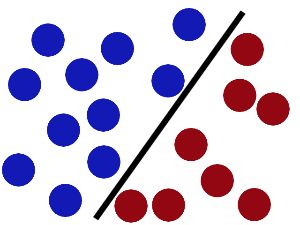
\includegraphics[width=0.5\linewidth]{partition/img/svm_6.jpg}  
%	\caption{this is a figure demo}
%	\label{fig:label}
	\end{figure}

\end{frame} 

\begin{frame}
\frametitle{一个游戏}	
 我们已经学会了一个trick,然后,在SVM 工具箱中有另一个更加重要的 trick,于是又有一个新的挑战。
           
	\begin{figure}[ht]
	\centering
	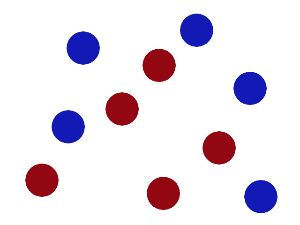
\includegraphics[width=0.5\linewidth]{partition/img/svm_7.jpg}  
%	\caption{this is a figure demo}
%	\label{fig:label}
	\end{figure}

\end{frame} 

\begin{frame}
\frametitle{一个游戏}	
现在,没有棍可以很好地分开两种球了,现在怎么办呢?我们可以一拍桌子,球飞到空中。然后,抓起一张纸,插到了两种球的中间。
           
	\begin{figure}[ht]
	\centering
	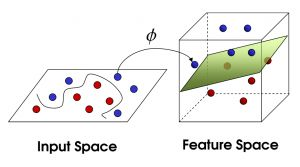
\includegraphics[width=0.5\linewidth]{partition/img/svm_8.jpg}  
%	\caption{this is a figure demo}
%	\label{fig:label}
	\end{figure}

\end{frame} 

\begin{frame}
\frametitle{一个游戏}	
现在,这些球看起来像是被一条曲线分开了。
           
	\begin{figure}[ht]
	\centering
	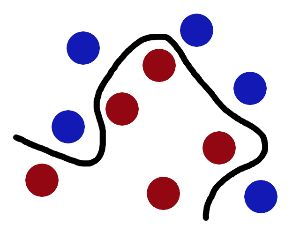
\includegraphics[width=0.5\linewidth]{partition/img/svm_9.jpg}  
%	\caption{this is a figure demo}
%	\label{fig:label}
	\end{figure}

\end{frame} 


\begin{frame}
\frametitle{怎么求解SVM?}
给定训练样本集$D = \{(x_1,y_1),(x_2,y_2),\dots,(x_m,y_m)\}$
 如果可以用一个线性超平面将其完全分开,那么这个超平面可以表示为:
\[\boldsymbol{w}^T\boldsymbol{x}+b=0\]
 其中$\boldsymbol{w}$决定了平面的方向,而b决定了平面与原点之间的距离。
           
	\begin{figure}[ht]
	\centering
	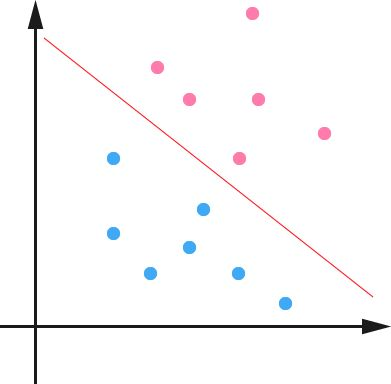
\includegraphics[width=0.5\linewidth]{partition/img/svm_10.jpg}  
%	\caption{this is a figure demo}
%	\label{fig:label}
	\end{figure}

\end{frame} 

\begin{frame}
\frametitle{间隔与支持向量}
空间中任意点$\boldsymbol{x}$实际上是一个向量,其到超平面的距离为:
\[r=\frac{\boldsymbol{w}^T\boldsymbol{x}+b}{\|\boldsymbol{w}\|}\]
	\begin{figure}[ht]
	\centering
	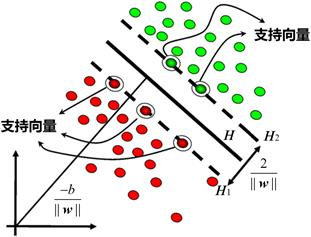
\includegraphics[width=0.5\linewidth]{partition/img/svm_11.jpg}  
%	\caption{this is a figure demo}
%	\label{fig:label}
	\end{figure}
\end{frame}

\begin{frame}
\frametitle{间隔与支持向量}
那么,如果这个超平面分类成功,我们令
\[\begin{cases}
\boldsymbol{w}^T\boldsymbol{x}+b\geq+1,\ y_i=+1\ ;\\
\boldsymbol{w}^T\boldsymbol{x}+b\leq-1,\ y_i=-1\ .
\end{cases} \]

	\begin{figure}[ht]
	\centering
	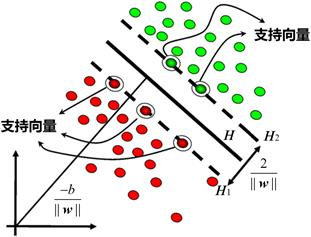
\includegraphics[width=0.5\linewidth]{partition/img/svm_11.jpg}  
%	\caption{this is a figure demo}
%	\label{fig:label}
	\end{figure}
\end{frame}

\begin{frame}
\frametitle{间隔与支持向量}

这样,那些使等号成立的点,也即距离超平面最近的点称作支持向量 (support vector),两个类到超平面距离之和也即两类之间的间隔 (margin) 是
\[
\gamma=\frac{2}{\|\boldsymbol{w}\|}
\]
训练支持向量机,实际上是希望找到具有最大间隔的划分超平面,即训练目标是在满足分类任务的情况下最大化$\gamma$,也即最大化$\|\boldsymbol{w}\|^{-1}$,也即最小化$\|\boldsymbol{w}\|^2$。
SVM的基本型就是:

\begin{gather*}
\min\limits_{\boldsymbol{w},b} \frac{1}{2}\|\boldsymbol{w}\|^2\\
s.t.\ y_i(\boldsymbol{w}^T\boldsymbol{x}_i+b)\geq1,\ i=1,2,\dots,m
\end{gather*}

%	\begin{figure}[ht]
%	\centering
%	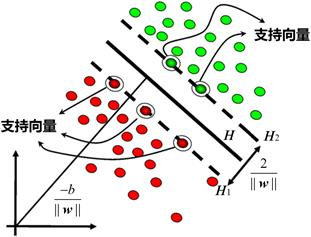
\includegraphics[width=0.3\linewidth]{partition/img/svm_11.jpg}  
%%	\caption{this is a figure demo}
%%	\label{fig:label}
%	\end{figure}
\end{frame}

\begin{frame}
\frametitle{对偶问题}
SVM的基本型是一个凸二次规划问题,可用现成的优化计算进行求解,求解的参数主要是$\boldsymbol{w}$ 和$b$。但我们可以有更高效的算法。使用拉格朗日乘子法可得到对偶问题,具体来说,对每条约束添加拉格朗日乘子$\alpha_i \ge0$,则该函数的拉格朗日函数可写为:
\[
\mathcal{L}(\boldsymbol{w},b,\boldsymbol{\alpha})=\frac{1}{2}\|\boldsymbol{w}\|^2-\sum_{i=1}^n\alpha_i \left(y_i(\boldsymbol{w}^T\boldsymbol{x_i}+b)-1\right)
\]
其中$\boldsymbol{\alpha} = (\alpha_1;\alpha_2;\dots;\alpha_m)$.令$\mathcal{L}(\boldsymbol{w},b,\boldsymbol{\alpha})$对$\boldsymbol{w}$和$b$的偏导为零可得
\begin{align*}
\boldsymbol{w} &= \sum_{i=1}^n\alpha_i y_i \boldsymbol{x}_i\ ,\\
0&=\sum_{i=1}^m\alpha_iy_i\ .
\end{align*}

\end{frame}


\begin{frame}

\frametitle{对偶问题}

将$\boldsymbol{w}$结果代入,即可将$\mathcal{L}(\boldsymbol{w},b,\boldsymbol{\alpha})$中的$\boldsymbol{w}$和$b$消去,再考虑第二个式子的约束,得到对偶问题:

\begin{align*}
 \max_\alpha &\sum_{i=1}^m\alpha_i – \frac{1}{2}\sum_{i=1}^m\sum_{j=1}^m\alpha_i\alpha_jy_iy_j\boldsymbol{x_i}^T\boldsymbol{x_j} \\ 
 s.t.,&\sum_{i=1}^m\alpha_iy_i = 0 \\
  &\alpha_i\geq 0, i=1,2,\ldots,m
 \end{align*}

解出$\boldsymbol{\alpha}$后,求出$\boldsymbol{w}$与$b$即可得到模型

\begin{align*}
f(x)&=\boldsymbol{w}^T\boldsymbol{x}+b\\
&=\sum_{i=1}^m\alpha_i y_i \boldsymbol{x_i}^T\boldsymbol{x}+b 
= \sum_{i=1}^m\alpha_i y_i \langle\boldsymbol{x_i, x}\rangle + b
\end{align*}

\end{frame}


\begin{frame}

\frametitle{对偶问题}
从对偶问题解出的$\alpha_i$是拉格朗日乘子,直接对应训练样本$(x_i,y_i)$。由于有不等式约束,因此上述过程需要满足KKT(Karush-Kuhn-Tucker)条件,即要求:
\[ 
\begin{cases}
\alpha_i \geq0\ ; \\
y_if(\boldsymbol{x_i})-1\geq 0\ ;\\
\alpha_i(y_if(\boldsymbol{x_i}-1)=0\ .
\end{cases} 
\]
于是,对于任意样本$(\boldsymbol{x_i},y_i)$总有$\alpha_i = 0$或$y_if(\boldsymbol{x_i})=1$。若$\alpha_i = 0$则该样本不会在求和中出现,若$\alpha_i > 0$,则必有$y_if(\boldsymbol{x_i})=1$,所对应的样本点位于最大间隔边上,是一个支持向量。也就是说,训练完成后,大部分的训练样本都不需要保留,最终模型仅与支持向量有关。
\end{frame}


\begin{frame}

\frametitle{SMO算法}
现在,回过头看问题转变成求解下式。这是一个二次规划问题,可以使用通用的二次规划算法来求解。这里可以使用更高效的算法,SMO算法。
\begin{align*}
 \max_\alpha &\sum_{i=1}^m\alpha_i – \frac{1}{2}\sum_{i=1}^m\sum_{j=1}^m\alpha_i\alpha_jy_iy_j\boldsymbol{x_i}^T\boldsymbol{x_j} \\ 
 s.t.,&\sum_{i=1}^m\alpha_iy_i = 0 \\
  &\alpha_i\geq 0, i=1,2,\ldots,m
 \end{align*}
其基本思想很简单:在每一步优化中,挑选出诸多参数$\alpha_k(k=1,2,...,N)$中的两个参数$\alpha_i,\alpha_j$作为“真正的参数”,其余参数都视为常数,从而我们就能求出解析解。

\end{frame}

\begin{frame}

\frametitle{SMO算法}

其大致求解步骤则可以概括如下:
	\begin{itemize}
		\item 选出$\alpha_1,\alpha_2,...,\alpha_N$中“最不好的”两个参数$\alpha_i、\alpha_j$
		\item 只把$\alpha_i,\alpha_j$视为参数并把其余的$\alpha_k$视为常数,于是最大化$\mathcal{L}(\alpha)$就变成了以$\alpha_i,\alpha_j$为参数的二次规划问题,从而可以直接对其进行求解。但是,注意到$\alpha_i,\alpha_j$需满足$\sum_{i=1}^N\alpha_iy_i=0$和$0\le\alpha_i,\alpha_j\le C$,所以求完解后需要检查是否满足约束;如不满足,则进行调整。
	\end{itemize}
 \vspace{1em}
SMO先选取违背KKT条件程度最大的变量。第二个变量应选择使目标函数值减小最快的变量,但是由于比较各变量对应目标函数值减幅的复杂度过高。SMO采用了一个启发式:使选取的两变量所对应的样本之间间隔最大。这样的两个变量有很大差别,与对两个相似变量进行更新相比,对他们进行更新会带给目标函数值更大的变化。
\end{frame}

\begin{frame}

\frametitle{SMO算法}
SMO之所以高效,是因为固定其他参数后,仅优化两个参数的过程非常高效,仅考虑$\alpha_i,\alpha_j$时,约束可以重写为
\[
\alpha_iy_i+\alpha_jy_j= c,\alpha_i>0,\alpha_j>0,
\]
其中
\[
c = -\sum_{k!=i,j}alpha_ky_k
\]
是使$\sum_{i=1}^m\alpha_iy_i=0$成立的常数,利用第一个式子消去$alpha_j$,则得到一个关于$\alpha_i$的单变量二次规划问题,仅有的约束是$\alpha_i\ge0$。这样的二次规划问题具有闭式解,于是不必调用数值优化算法即可高效地计算出更新后的$\alpha_i,\alpha_j$。\\
然后使用所有支持向量求解偏移项的平均值作为b.


\end{frame}

\begin{frame}

\frametitle{核函数}

    我们上面得到的SVM只能处理线性的问题,并不能处理非线性的问题,如果需要解决这种问题,那么其实就需要将低维数据转化到高维空间,从而找到一个超平面将其分割开来。简单的说,我们需要找到一个函数,可以将我们的原始特征通过这个函数进行映射。\\
    我们前面得到的函数形式是:
 \[
 f(x)= \sum_{i=1}^m\alpha_i y_i \langle\boldsymbol{x_i, x}\rangle + b
 \]
 则映射过后变成:  
  \[
 f(x)= \sum_{i=1}^m\alpha_i y_i \langle\boldsymbol{\phi(x_i),\phi(x)}\rangle + b
 \]

\end{frame}


\begin{frame}

\frametitle{核函数}

同样的求解形式:
\begin{align*}
 \max_\alpha &\sum_{i=1}^m\alpha_i – \frac{1}{2}\sum_{i=1}^m\sum_{j=1}^m\alpha_i\alpha_jy_iy_j\langle\boldsymbol{\phi(x_i)},\boldsymbol{\phi(x_j)}\rangle \\ 
 s.t.,&\sum_{i=1}^m\alpha_iy_i = 0 \\
  &\alpha_i\geq 0, i=1,2,\ldots,m
 \end{align*}

 很直接的想法是,先通过$\phi(x)$将x映射到高维空间,然后再做内积运算,但在这种运算方式并不推荐,二维空间如果选择一阶二阶的组合就有5个维度,如果将维数和组合复杂度提高的话,那么映射的空间维度就会爆炸性的增长,从而为计算带来了很大的困难。那么此时我们就可以用核函数的方法来解决这类问题.
\end{frame}


\begin{frame}

\frametitle{核函数}

可以设想这样的一个函数:
\[
\kappa(\boldsymbol{x_i,x_j})=\langle\boldsymbol{\phi(x_i),\phi(x_j)}\rangle = \phi(\boldsymbol{x_i})^T\phi(\boldsymbol{x_j})
\]

即$\boldsymbol{x_i}$和$\boldsymbol{x_j}$在特征空间的内积等于他们在原始样本空间中通过函数$\kappa(\cdot,\cdot)$计算的结果.有了这样的函数,我们就不必去计算高维甚至无穷维特征空间中的内积。于是求解式可以重写为:
\begin{align*}
 \max_\alpha &\sum_{i=1}^m\alpha_i – \frac{1}{2}\sum_{i=1}^m\sum_{j=1}^m\alpha_i\alpha_jy_iy_j\kappa(\boldsymbol{x_i,x_j}) \\ 
 s.t.,&\sum_{i=1}^m\alpha_iy_i = 0 \\
  &\alpha_i\geq 0, i=1,2,\ldots,m
 \end{align*}
\end{frame}


\begin{frame}

\frametitle{核函数}

求解后即可得到:
\begin{align*}
f(x)&=\boldsymbol{w}^T\phi(\boldsymbol{x})+b\\
&=\sum_{i=1}^m\alpha_i y_i \phi(\boldsymbol{x_i})^T\phi(\boldsymbol{x})+b\\
&= \sum_{i=1}^m\alpha_i y_i \kappa(\boldsymbol{x_i, x}) + b
\end{align*}
\end{frame}


\begin{frame}

\frametitle{核函数}

定理 (核函数):
令$\chi$为输入空间,$\kappa(\cdot,\cdot)$是定义在$\chi\times\chi$上的对称函数,则$\kappa$是核函数当且仅当对于任意数据$D={x_1,x_2,...,x_m}$,只要对称函数所对应的核矩阵半正定,它就能作为核函数使用;反之,对于一个半正定核矩阵,总能找到一个与之对应的映射$\phi$。任何一个核函数隐式地定义了一个称为“再生核希尔伯特空间”(Reproducing Kernel Hilbert Space,RKHS)的特征空间。

 \begin{table}[ht]
%  \caption{test}
%  \label{Tab:bookRWCal}

\begin{tabular}{l|l|l}

名称 & 表达式 & 参数\\  
线性核 &$\kappa(\boldsymbol{x_i,x_j})=\boldsymbol{x_i}^T\boldsymbol{x_j}$ &  \\ 
多项式核 &$\kappa(\boldsymbol{x_i,x_j})=(\boldsymbol{x_i}^T\boldsymbol{x_j})^d$ & $d\ge1$为多项式的次数 \\  
高斯核 & $\kappa(\boldsymbol{x_i,x_j})=exp(-\frac{\lVert x_i-x_j\rVert^2}{2\sigma^2})$ & $\sigma\ge0$为高斯核的带宽 \\  
拉普拉斯核 &  $\kappa(\boldsymbol{x_i,x_j})=exp(-\frac{\lVert x_i-x_j\rVert}{\sigma})$ &$\sigma\ge0$ \\  
Sigmoid核&$tanh(\beta\boldsymbol{x_i}^T\boldsymbol{x_j}+\theta)$ &$\beta>0,\theta<0$\\
\end{tabular}  
\end{table}

\end{frame}


\begin{frame}

\frametitle{软间隔}
 在很多实际问题,由于存在各种噪音,所以现实生活中的分类可能并不能直接通过一个超平面将其完全分隔开来,即使能完全分隔,但得到的超平面也不一定是最佳的,如图中的情况。所以,我们需要对某些样本有一定的容忍度,允许他们跑到分隔区域中,那么原来的约束条件需要进行变化
 \begin{figure}[ht]
	\centering
	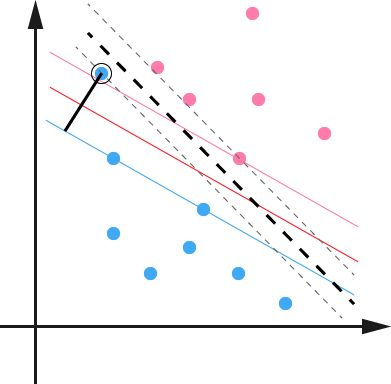
\includegraphics[width=0.5\linewidth]{partition/img/svm_12.jpg}  
%	\caption{this is a figure demo}
%	\label{fig:label}
	\end{figure}
 
\end{frame}


\begin{frame}

\frametitle{软间隔}
\[
y_i(w^Tx_i+b)\geq 1-\xi_i, \quad i=1,\ldots,n
\]
$\xi_i\geq 0$是一个松弛变量,即允许$ x_i$ 偏离的量,但同样的我们也要使 $\xi_i$ 的和最小,那么优化问题完整的写出来:

\begin{align*}
\min & \frac{1}{2}\|w\|^2 + C\sum_{i=1}^n\xi_i \\
 s.t., & y_i(w^Tx_i+b)\geq 1-\xi_i, i=1,\ldots,n \\
& \xi_i \geq 0, i=1,\ldots,n 
\end{align*}

其中C是一个预先设定的值,很明显,当C无穷大时,就代表了 $\xi_i=0$ ,即是之前的那种情况。

\end{frame}


\begin{frame}
\frametitle{软间隔}

用之前的方法可得:
\[
\mathcal{L}(w,b,\xi,\alpha,r)=\frac{1}{2}\|w\|^2 + C\sum_{i=1}^n\xi_i – \sum_{i=1}^n\alpha_i \left(y_i(w^Tx_i+b)-1+\xi_i\right) – \sum_{i=1}^n r_i\xi_i
\]

$\mathcal{L}(w,b,\xi,\alpha,r)$对$w,b,\xi_i$求偏导可得:

\begin{align*}
\frac{\partial \mathcal{L}}{\partial w}=0 &\Rightarrow w=\sum_{i=1}^n \alpha_i y_i x_i \\
\frac{\partial \mathcal{L}}{\partial b} = 0 &\Rightarrow \sum_{i=1}^n \alpha_i y_i = 0 \\
\frac{\partial \mathcal{L}}{\partial \xi_i} = 0 &\Rightarrow C-\alpha_i-r_i=0, \quad i=1,\ldots,n 
\end{align*}

\end{frame}


\begin{frame}
\frametitle{软间隔}

带回原式,可以看到目标函数并没有发生变化,但约束条件变了:

\begin{align*}
\max_\alpha &\sum_{i=1}^n\alpha_i – \frac{1}{2}\sum_{i,j=1}^n\alpha_i\alpha_jy_iy_j\langle x_i,x_j\rangle \\
s.t., &0\leq \alpha_i\leq C, i=1,\ldots,n \\
&\sum_{i=1}^n\alpha_iy_i = 0
\end{align*}
可采用之前同样的算法求解。
\end{frame}


\end{document}  